\section{Experimental Apparatus}

\subsection{The Large Hadron Collider}

\begin{frame}
\frametitle{The Large Hadron Collider}
\begin{columns}
\column{.5\textwidth}
\begin{itemize}
    \item The Large Hadron Collider (LHC) collides protons at a
        center-of-mass energy of $\sqrts = 8$~TeV.
    \item Protons flow through a series of linear and synchrotron
        acclerators before entering the LHC ring.
    \item Proton bunches circulate counter to each other in two
        beams and are crossed at four primary interaction points.
\end{itemize}
\column{.5\textwidth}
\begin{itemize}
    \item Bunch crossings occur every 50~ns; approximately 20
        interactions per bunch crossing (pile-up)
\end{itemize}
\vfill
\begin{figure}
\centering
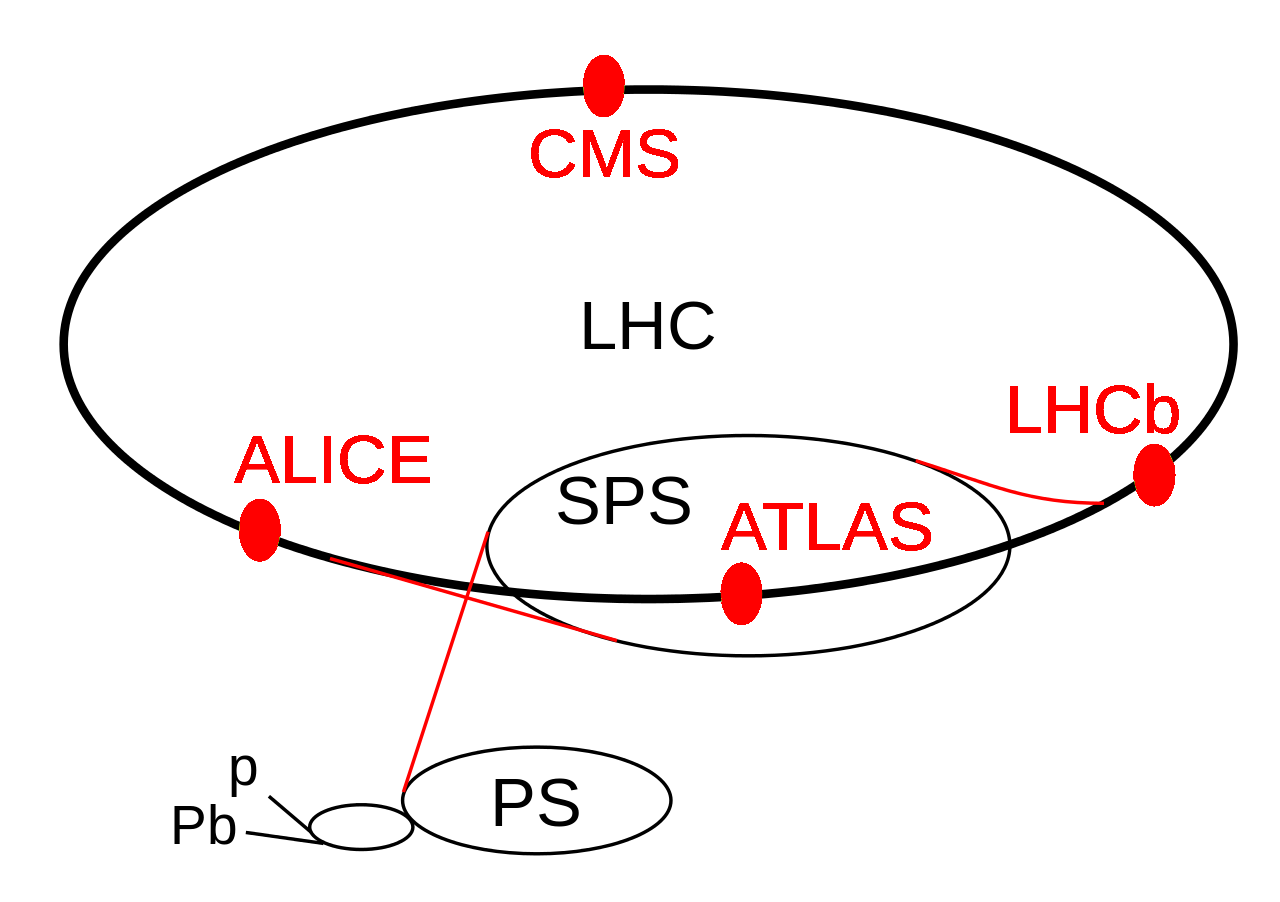
\includegraphics[width=\textwidth]{lhc.png}
\end{figure}
\end{columns}
\end{frame}

\subsection{The ATLAS Detector}

\begin{frame}
    \frametitle{ATLAS (A Toroidal LHC ApparatuS)}
\begin{figure}
\centering
\includegraphics[width=\textwidth]{atlas.eps}
\end{figure}
\end{frame}

\subsubsection{Coordinate Stystem}

\begin{frame}
\frametitle{Coordinate System}
\begin{itemize}
    \item $z$-axis along beam; $y$-axis points up; $x$-axis
        points to center of ring.
    \item Pseudorapidity $\eta = -\ln \tan(\theta/2)$; $\dr = \sqrt{\Delta \eta^2 + \Delta \phi^2}$
    \item small $|\eta| \to$ central ``barrel'' region; large
        $|\eta| \to$ forward ``end-caps''
    \item Transverse quantities (i.e. $p_T$, $E_T$) are projections
        onto the $x$-$y$ plane.
\end{itemize}
\begin{figure}
\centering
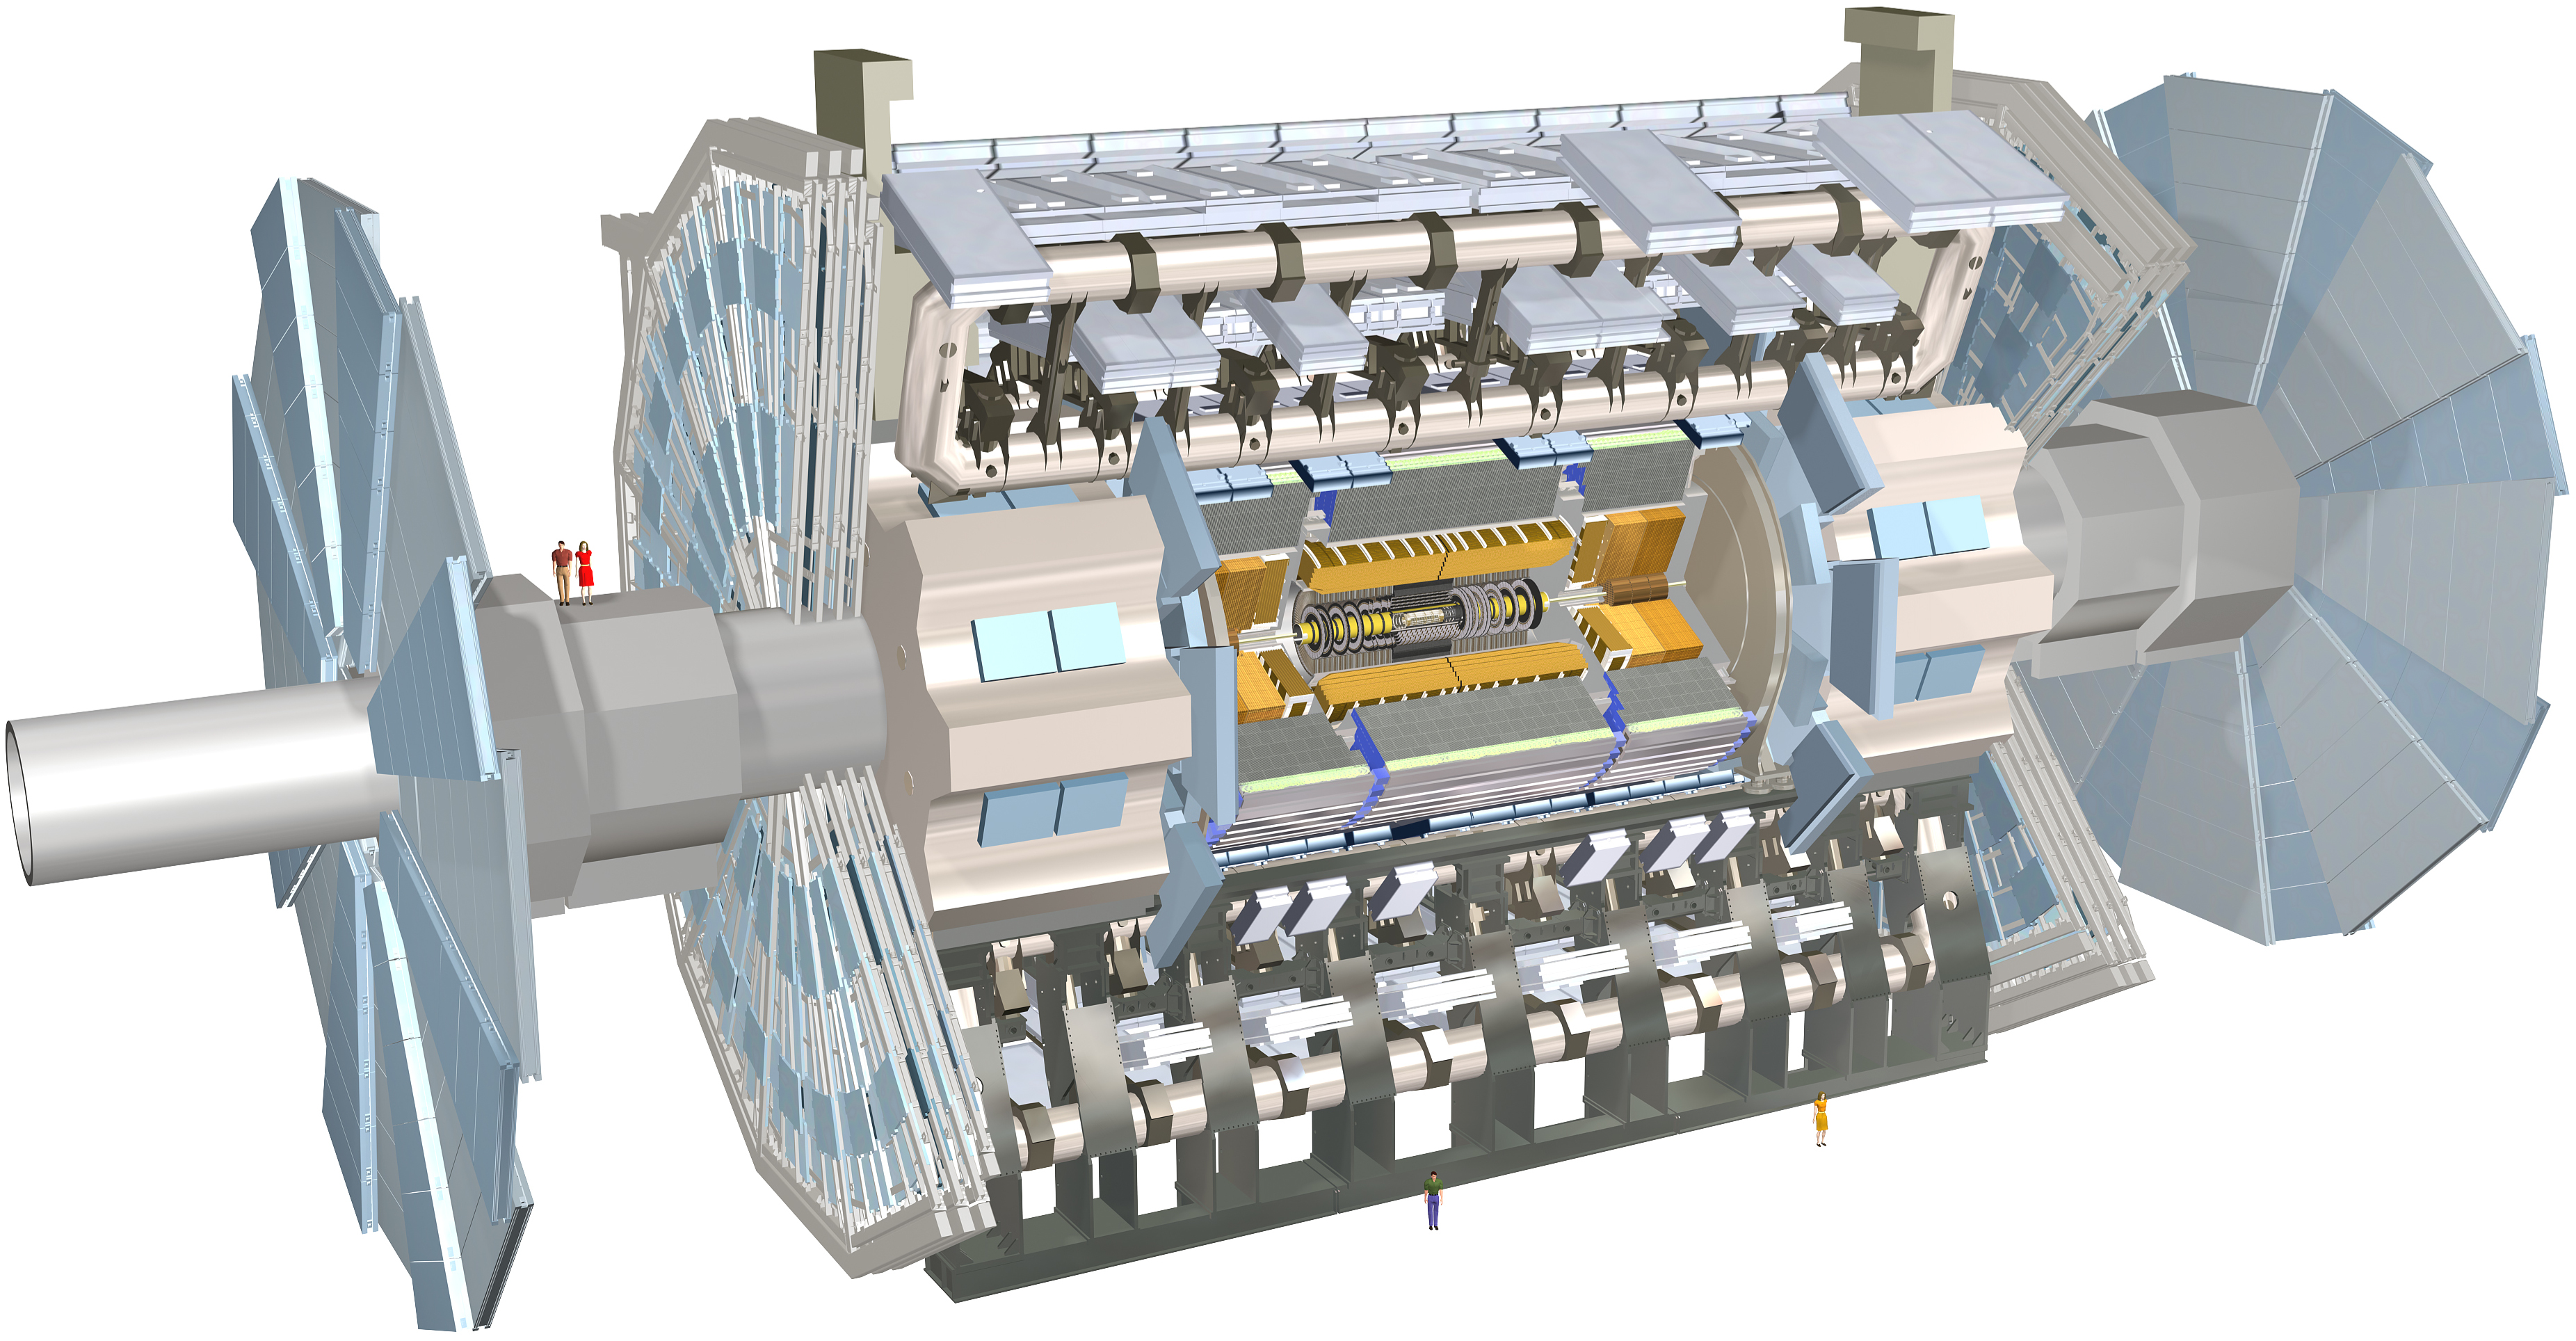
\includegraphics[height=5cm]{atlas_nolabel.jpg}
\end{figure}
\end{frame}


\subsubsection{Inner Detector}

\begin{frame}
\frametitle{Inner Detector}
\begin{columns}
\column{.5\textwidth}
\begin{figure}
\centering
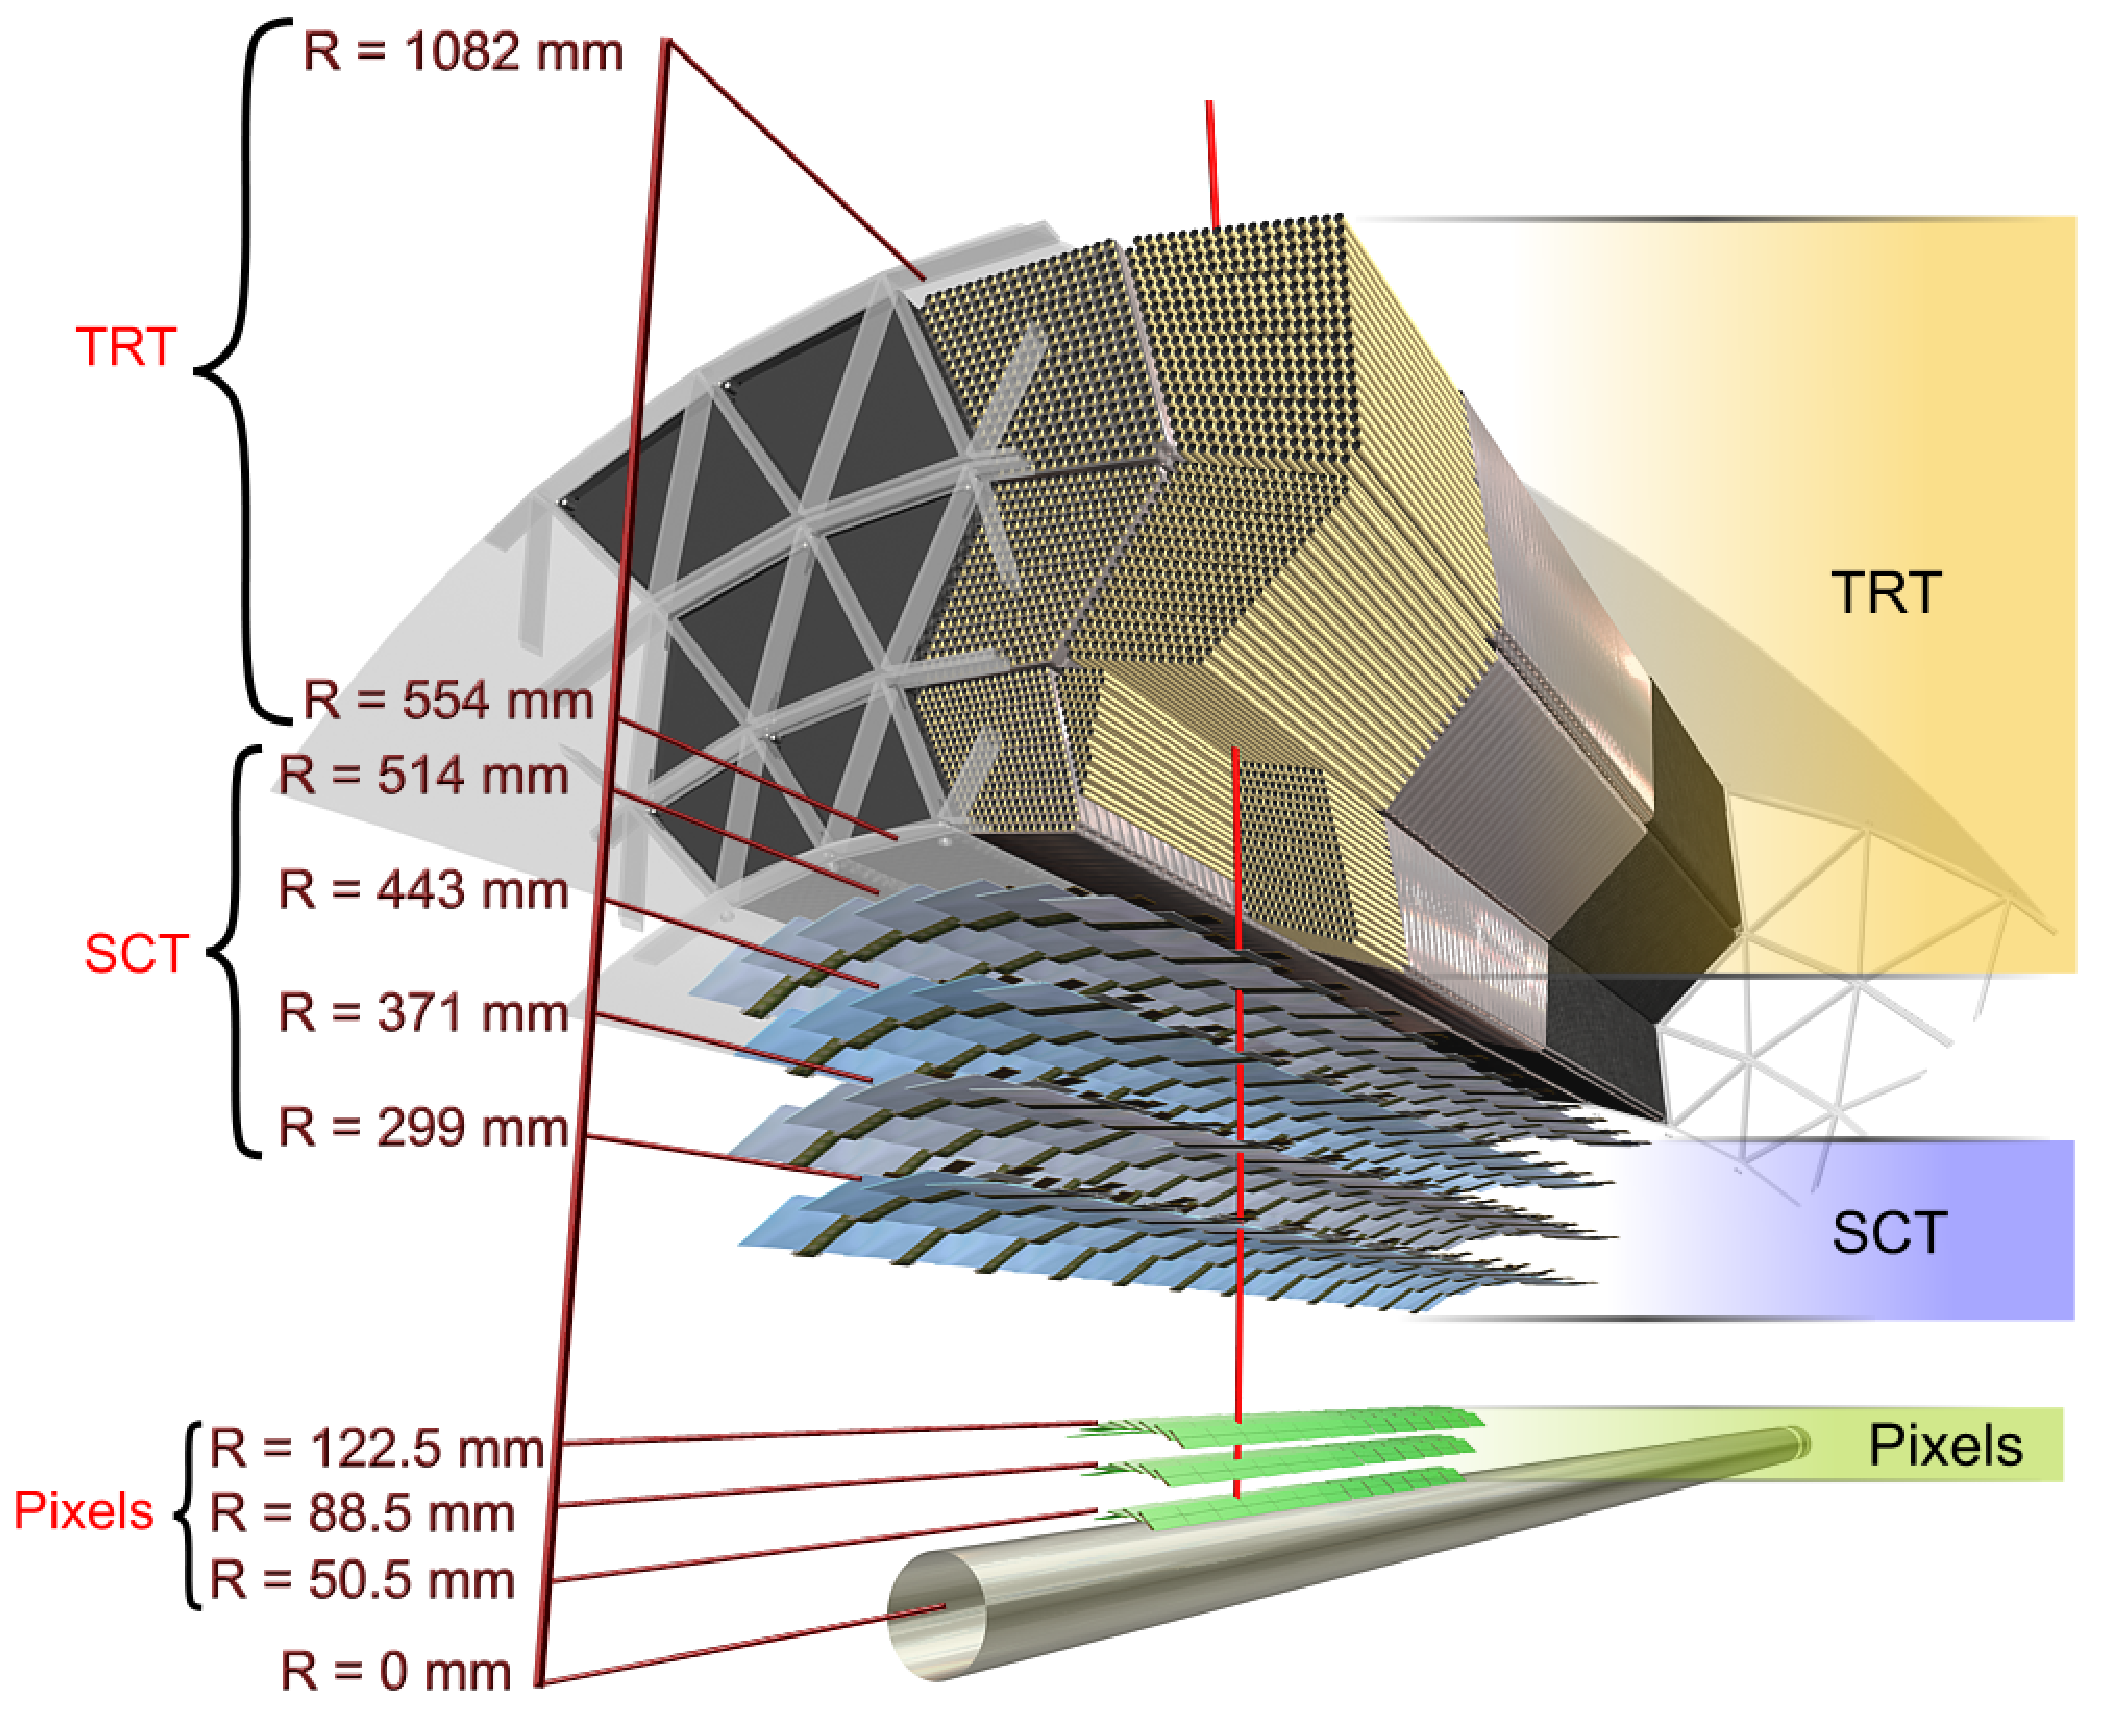
\includegraphics[width=\textwidth]{innerdetbarrel.eps}
\end{figure}
\column{.5\textwidth}
\begin{itemize}
    \item $\sim$1 meter in radial length
    \item Charged particles deposit energy (``hits'') in active
        detector elements.
    \item Surrounded by solenoid magnets which provide a uniform
        2~Tesla magnetic field, bending charge particle trajectories
    \item Three subsystems:
    \begin{itemize}
        \item Silicon Pixel Detector (pixels)
        \item Semiconductor Tracker (SCT)
        \item Transition Radiation Tracker (TRT)
    \end{itemize}
\end{itemize}
\end{columns}
\end{frame}

\subsubsection{Electromagnetic Calorimeter}

\begin{frame}
\centering
\frametitle{Electromagnetic Calorimeter}
\begin{figure}
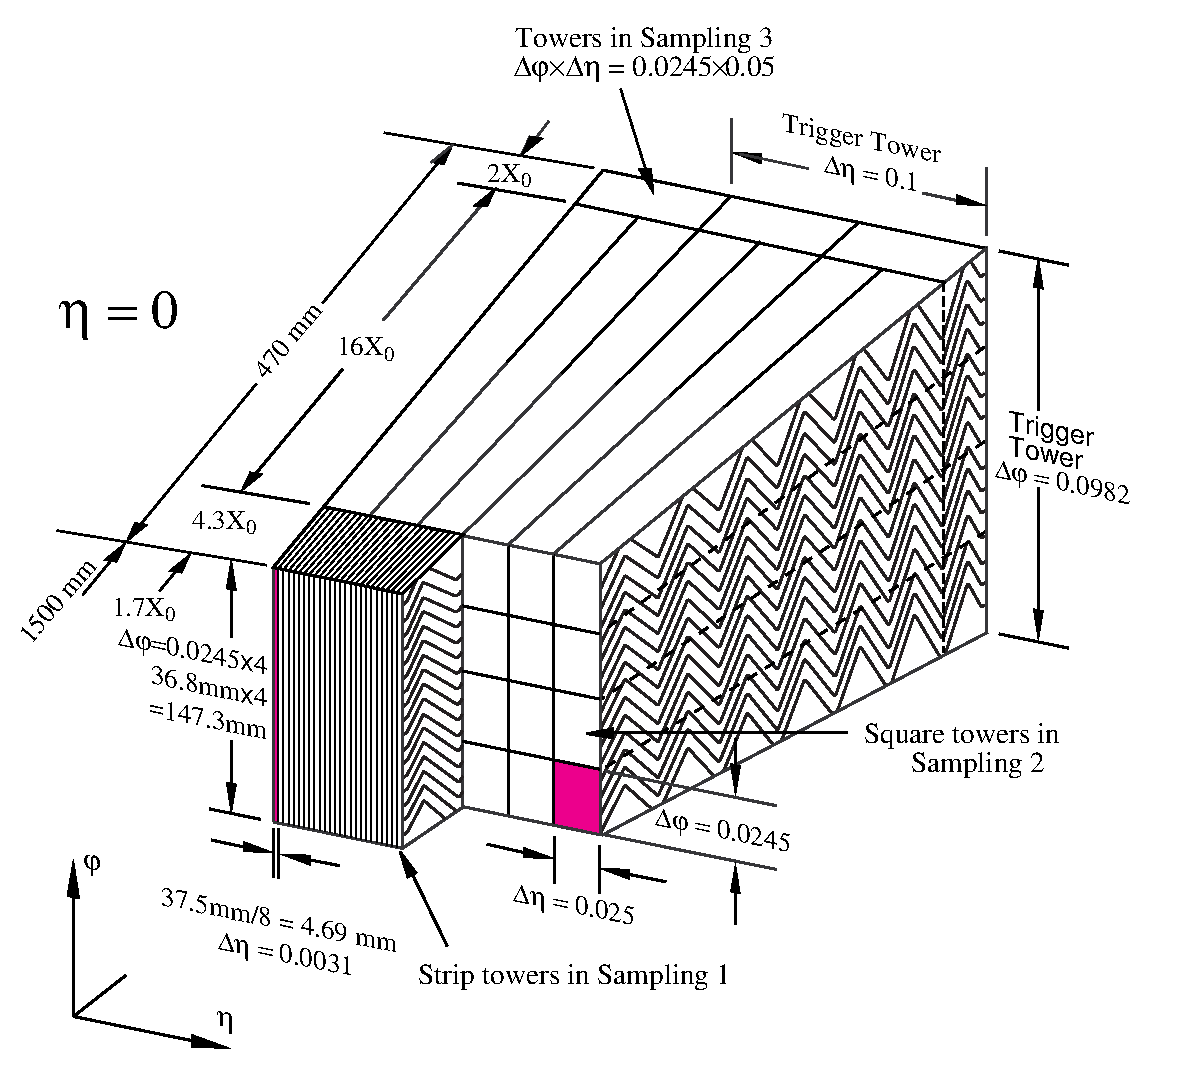
\includegraphics[height=4.5cm]{accordion.eps}
\end{figure}
\begin{itemize}
\item Alternating absorbing (lead) and active (liquid argon) layers
\item $|\eta| < 2.47$: precision region
\end{itemize}
\begin{equation*}
\frac{\sigma_E}{E} \approx \frac{10\%}{\sqrt{E/\mathrm{GeV}}} \oplus 0.7\%.
\end{equation*}
\end{frame}

\subsubsection{Hadronic Calorimeter}

\begin{frame}
\centering
\frametitle{Hadronic Calorimeter}
\begin{figure}
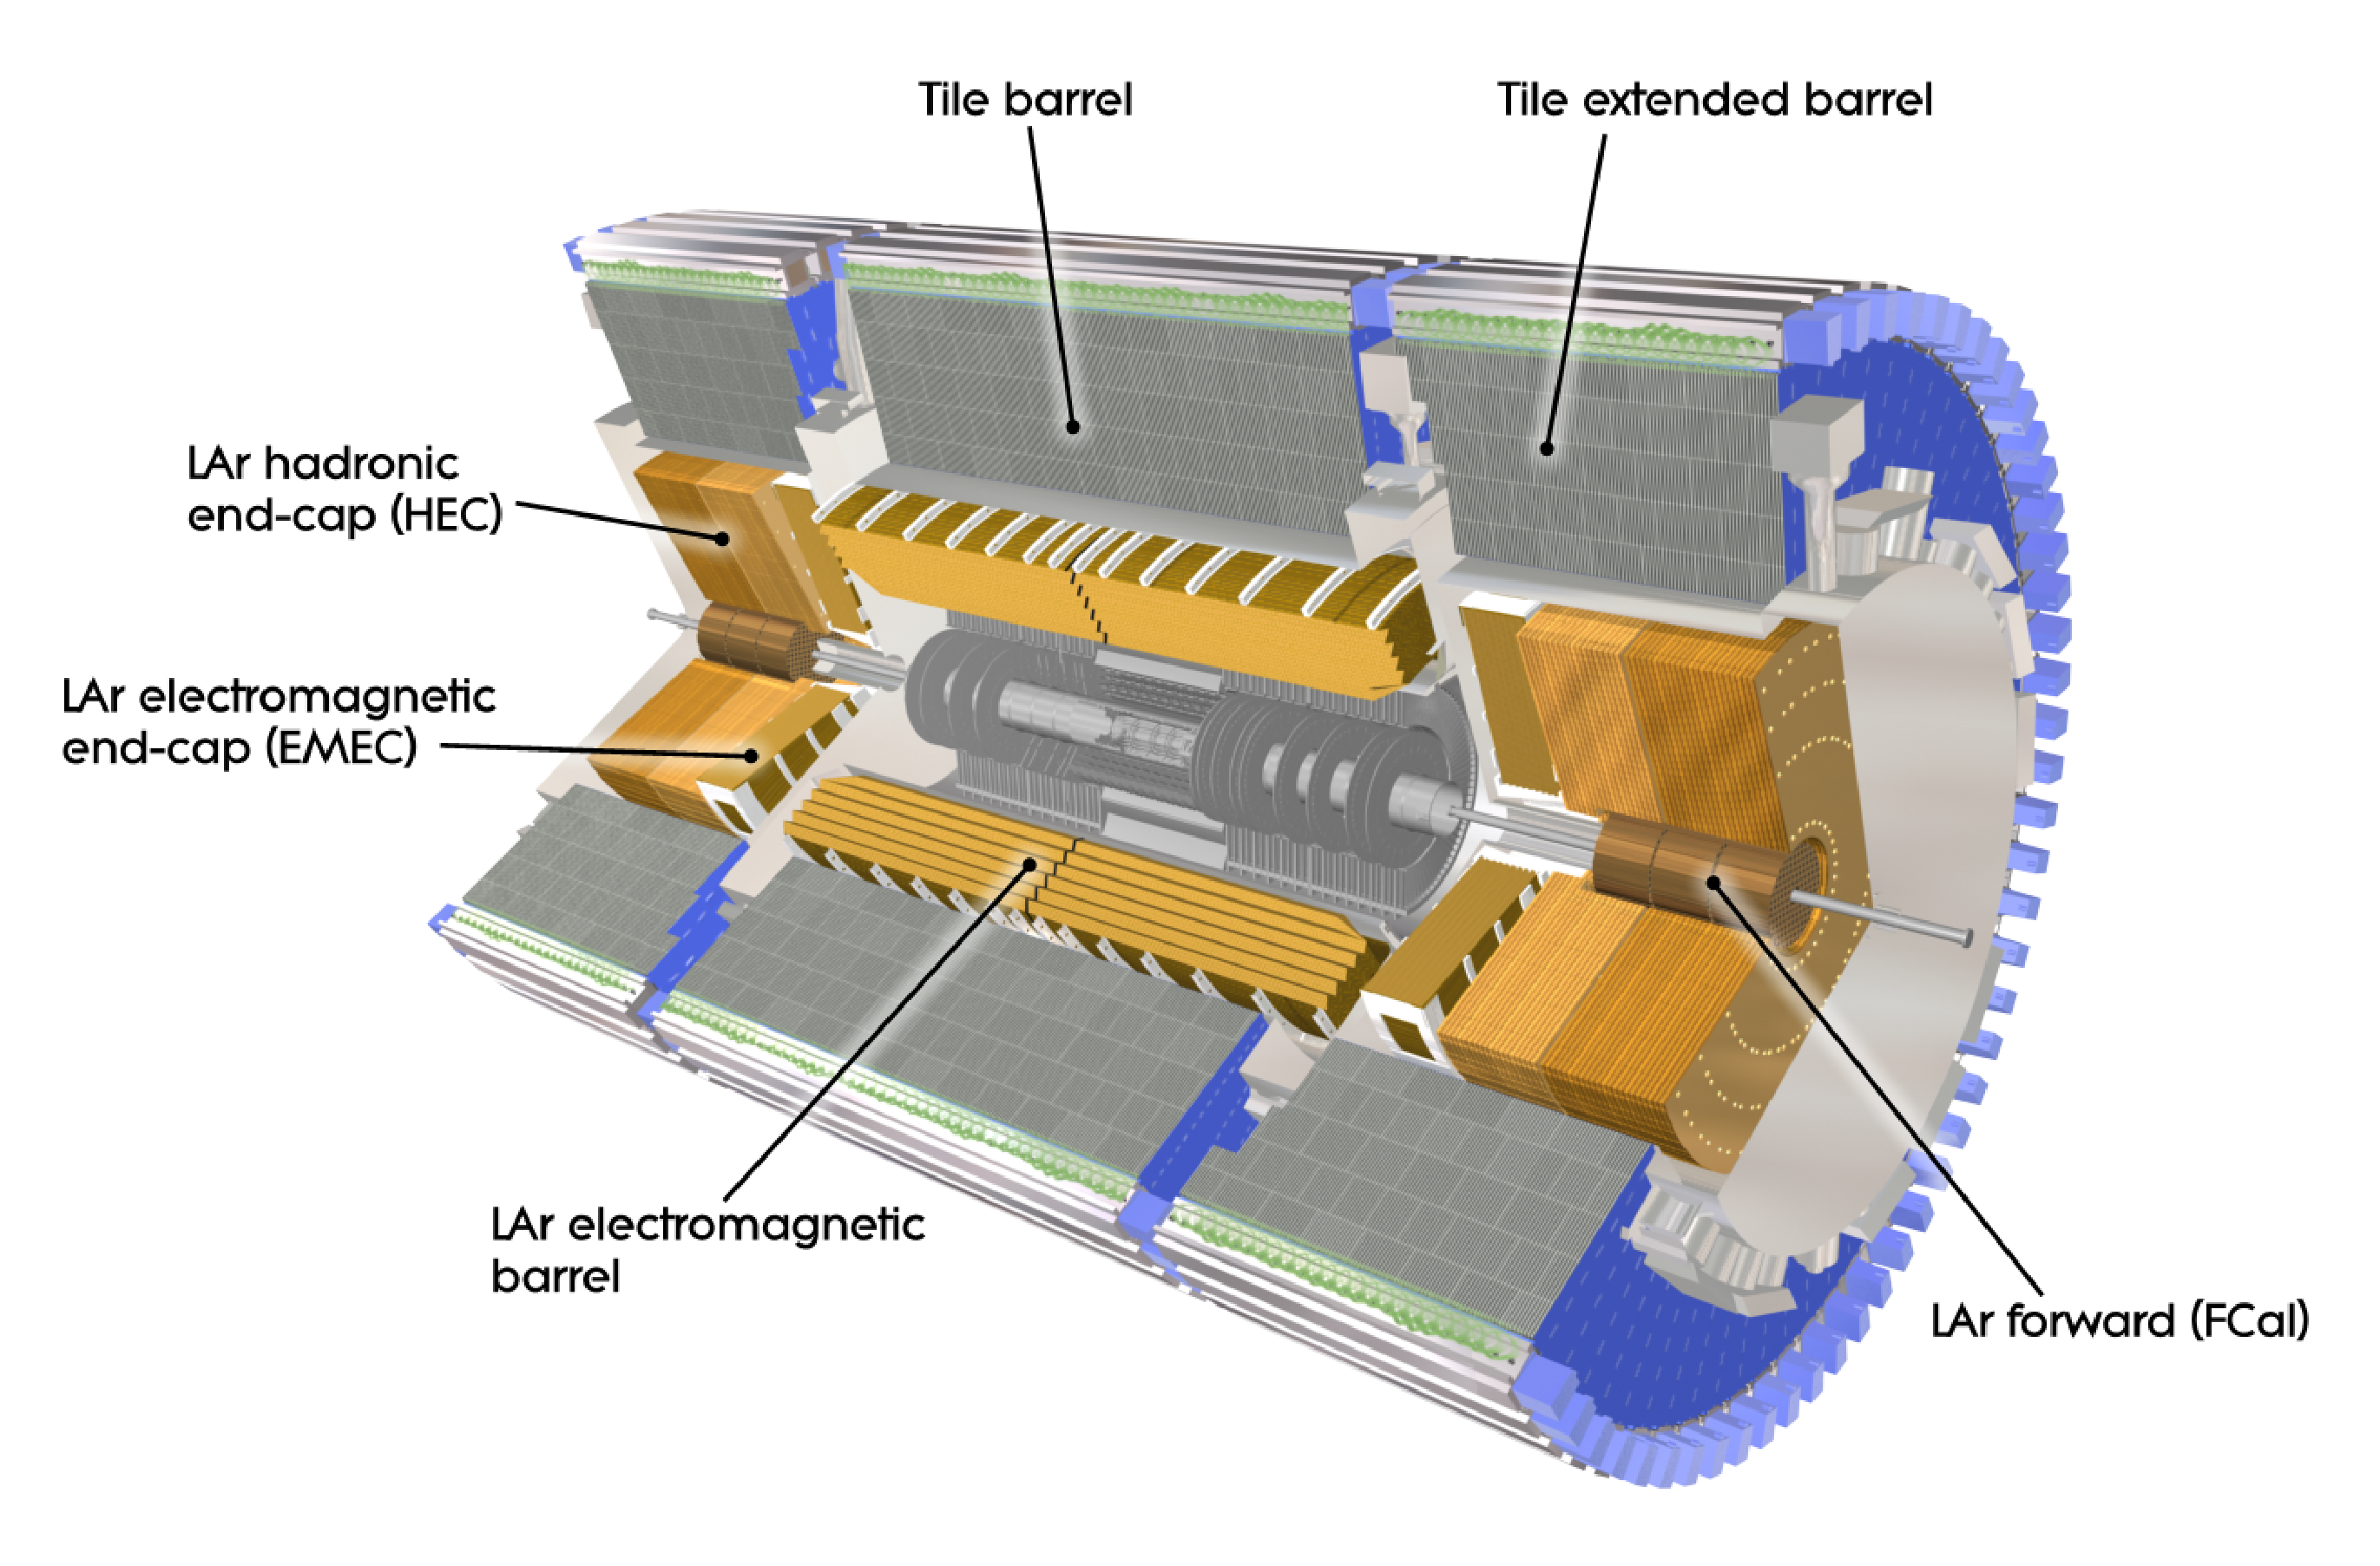
\includegraphics[height=5cm]{calorimeters.eps}
\end{figure}
\begin{itemize}
    \item Tile calorimeter: $|\eta| < 1.7$; steel absorber and
        scintilating tiles
    \item End-cap calorimeter: $1.5 < |\eta| < 3.2$; copper and liquid
        argon
    \item Forward calorimeter: $3.1 < |\eta| < 4.9$; copper/tungsten and
        liquid argon
\end{itemize}
\end{frame}

\subsubsection{Muon System}

\begin{frame}
\centering
\frametitle{Muon System}
\begin{figure}
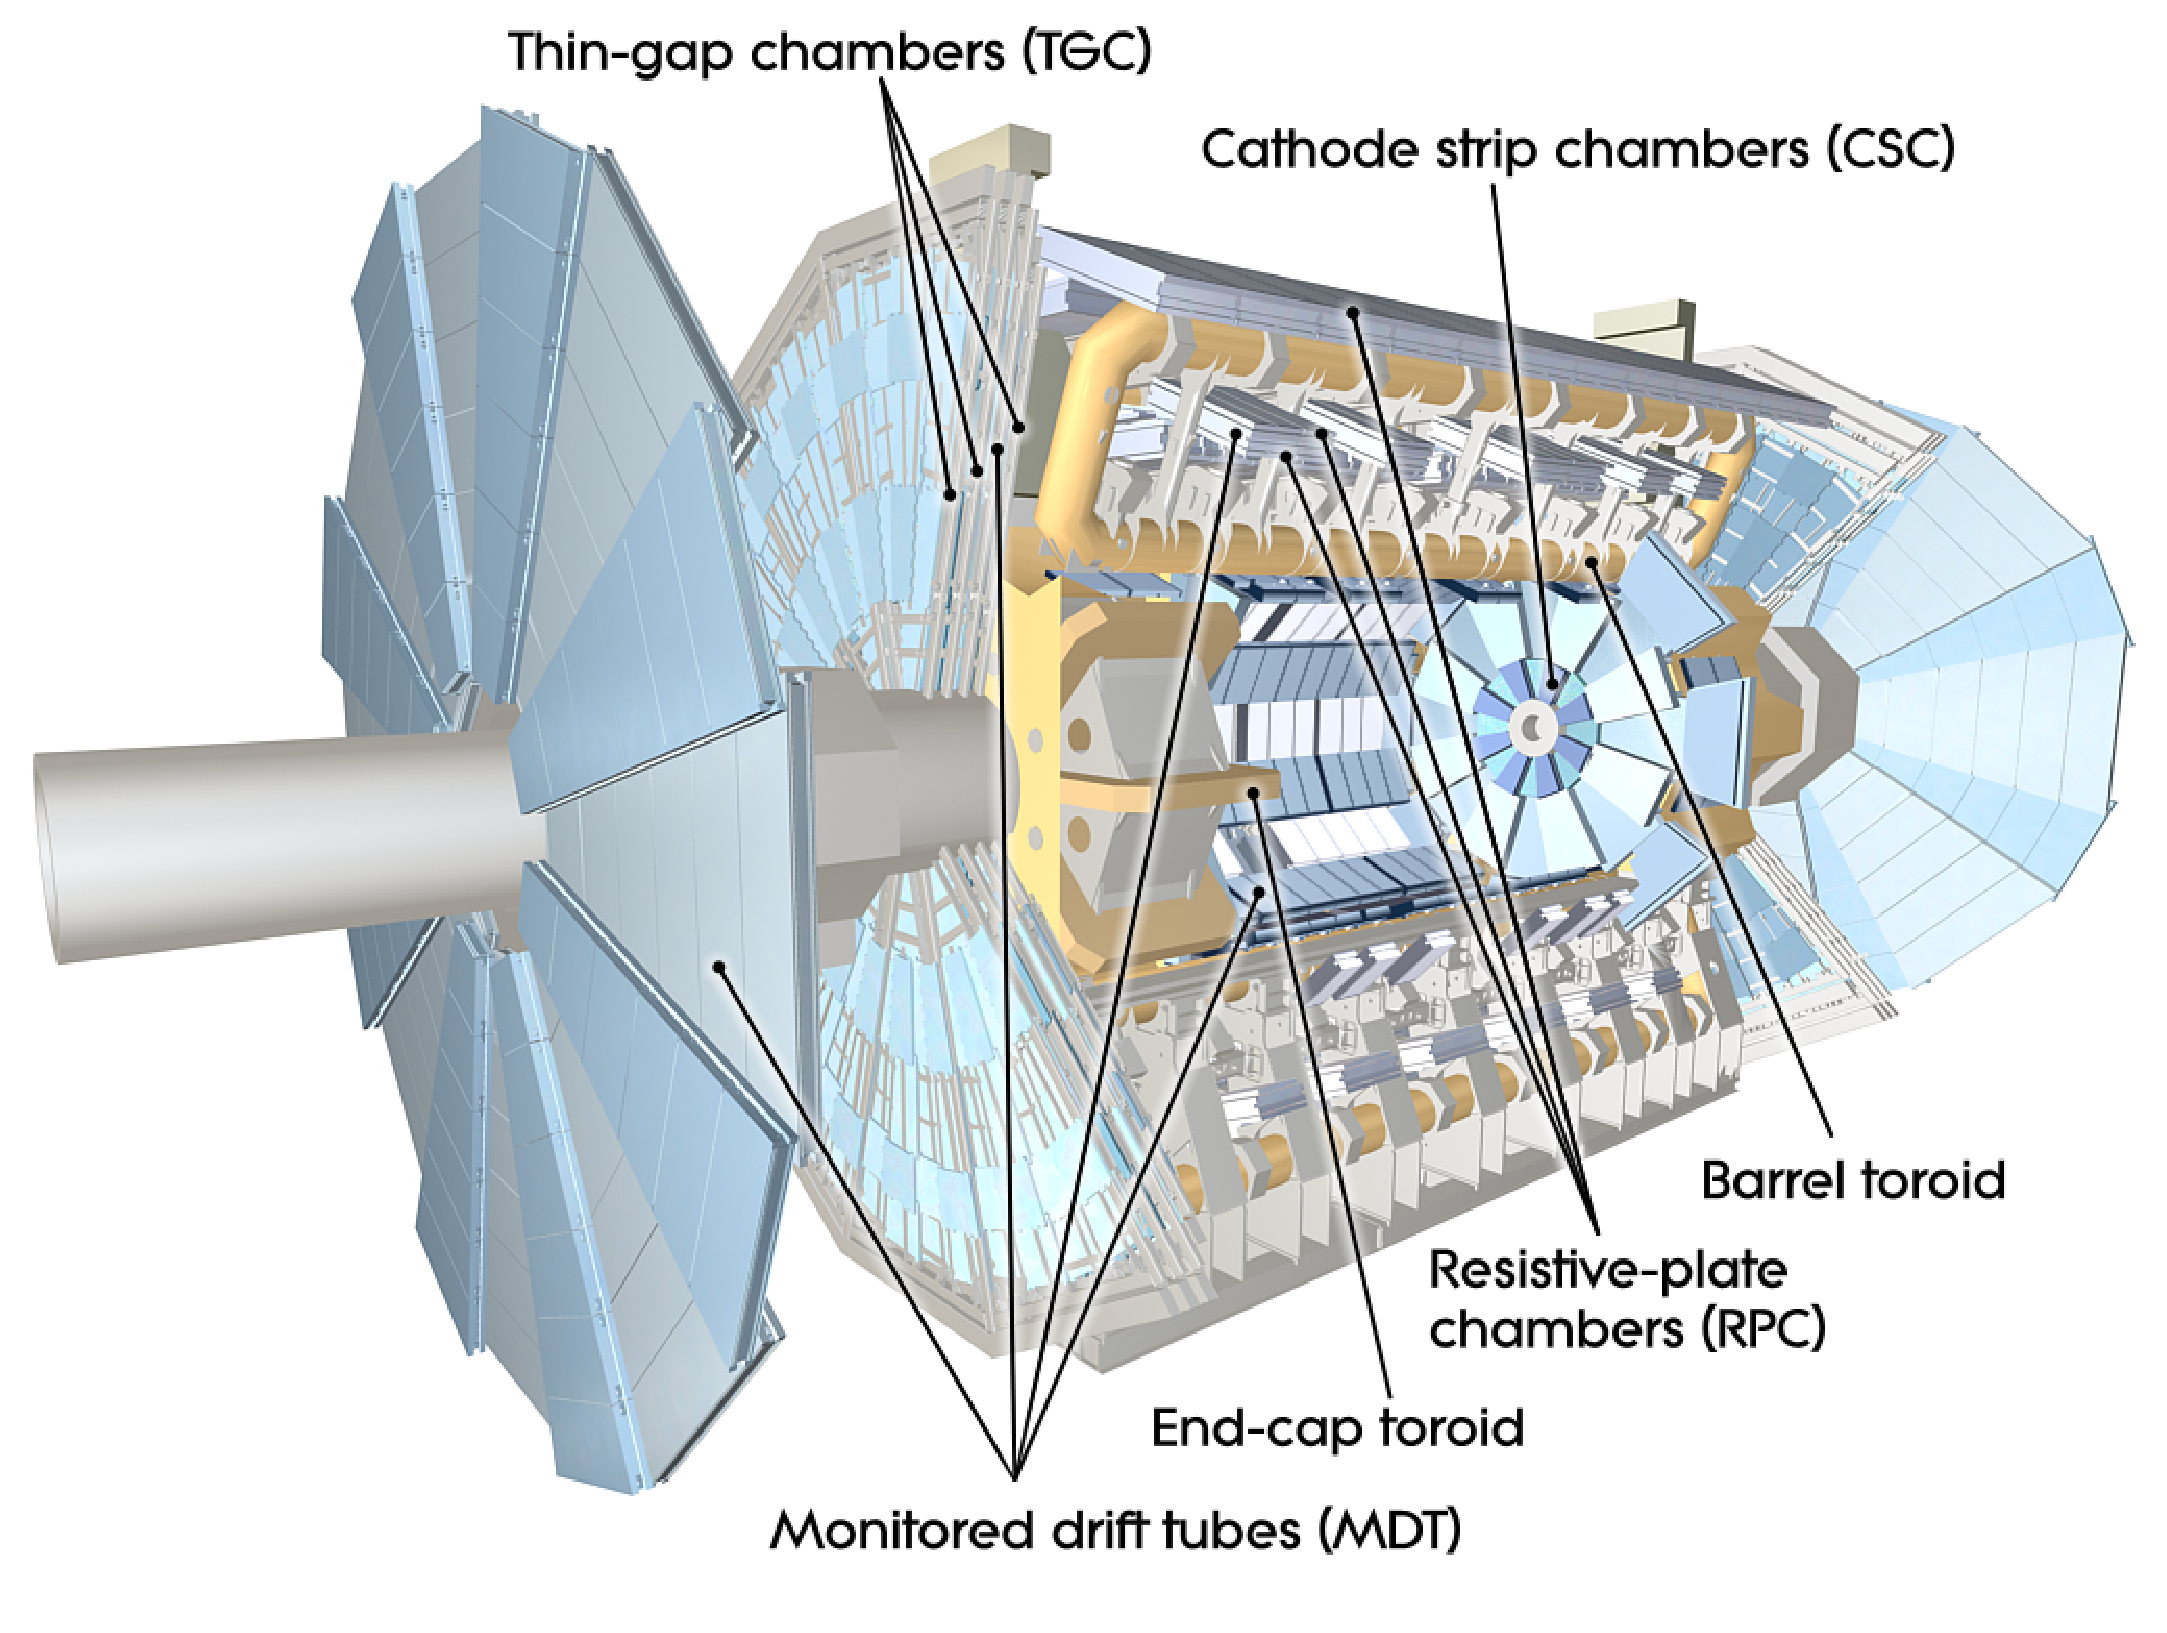
\includegraphics[height=4.5cm]{muonsystem.eps}
\end{figure}
\begin{itemize}
\item Outermost subdetector system at ATLAS
\item Surrounded by toroid magnet to bend muon trajectories
\item Three layers of trackers with a combination of fast readout and
    good momentum resolution
\end{itemize}
\end{frame}

\subsection{Simulation}

\begin{frame}
\frametitle{Event Simulation}

\centering
Monte Carlo (MC) used to predict the kinematics of proton collisions

\begin{columns}
    \column{.5\textwidth}
\begin{itemize}
\item Event generators $\to$ hard parton-parton scatter
\item Parton shower generators $\to$ QCD shower and hadronization
\item \geant4 $\to$ detector interactions
\end{itemize}

    \column{.5\textwidth}
\begin{figure}
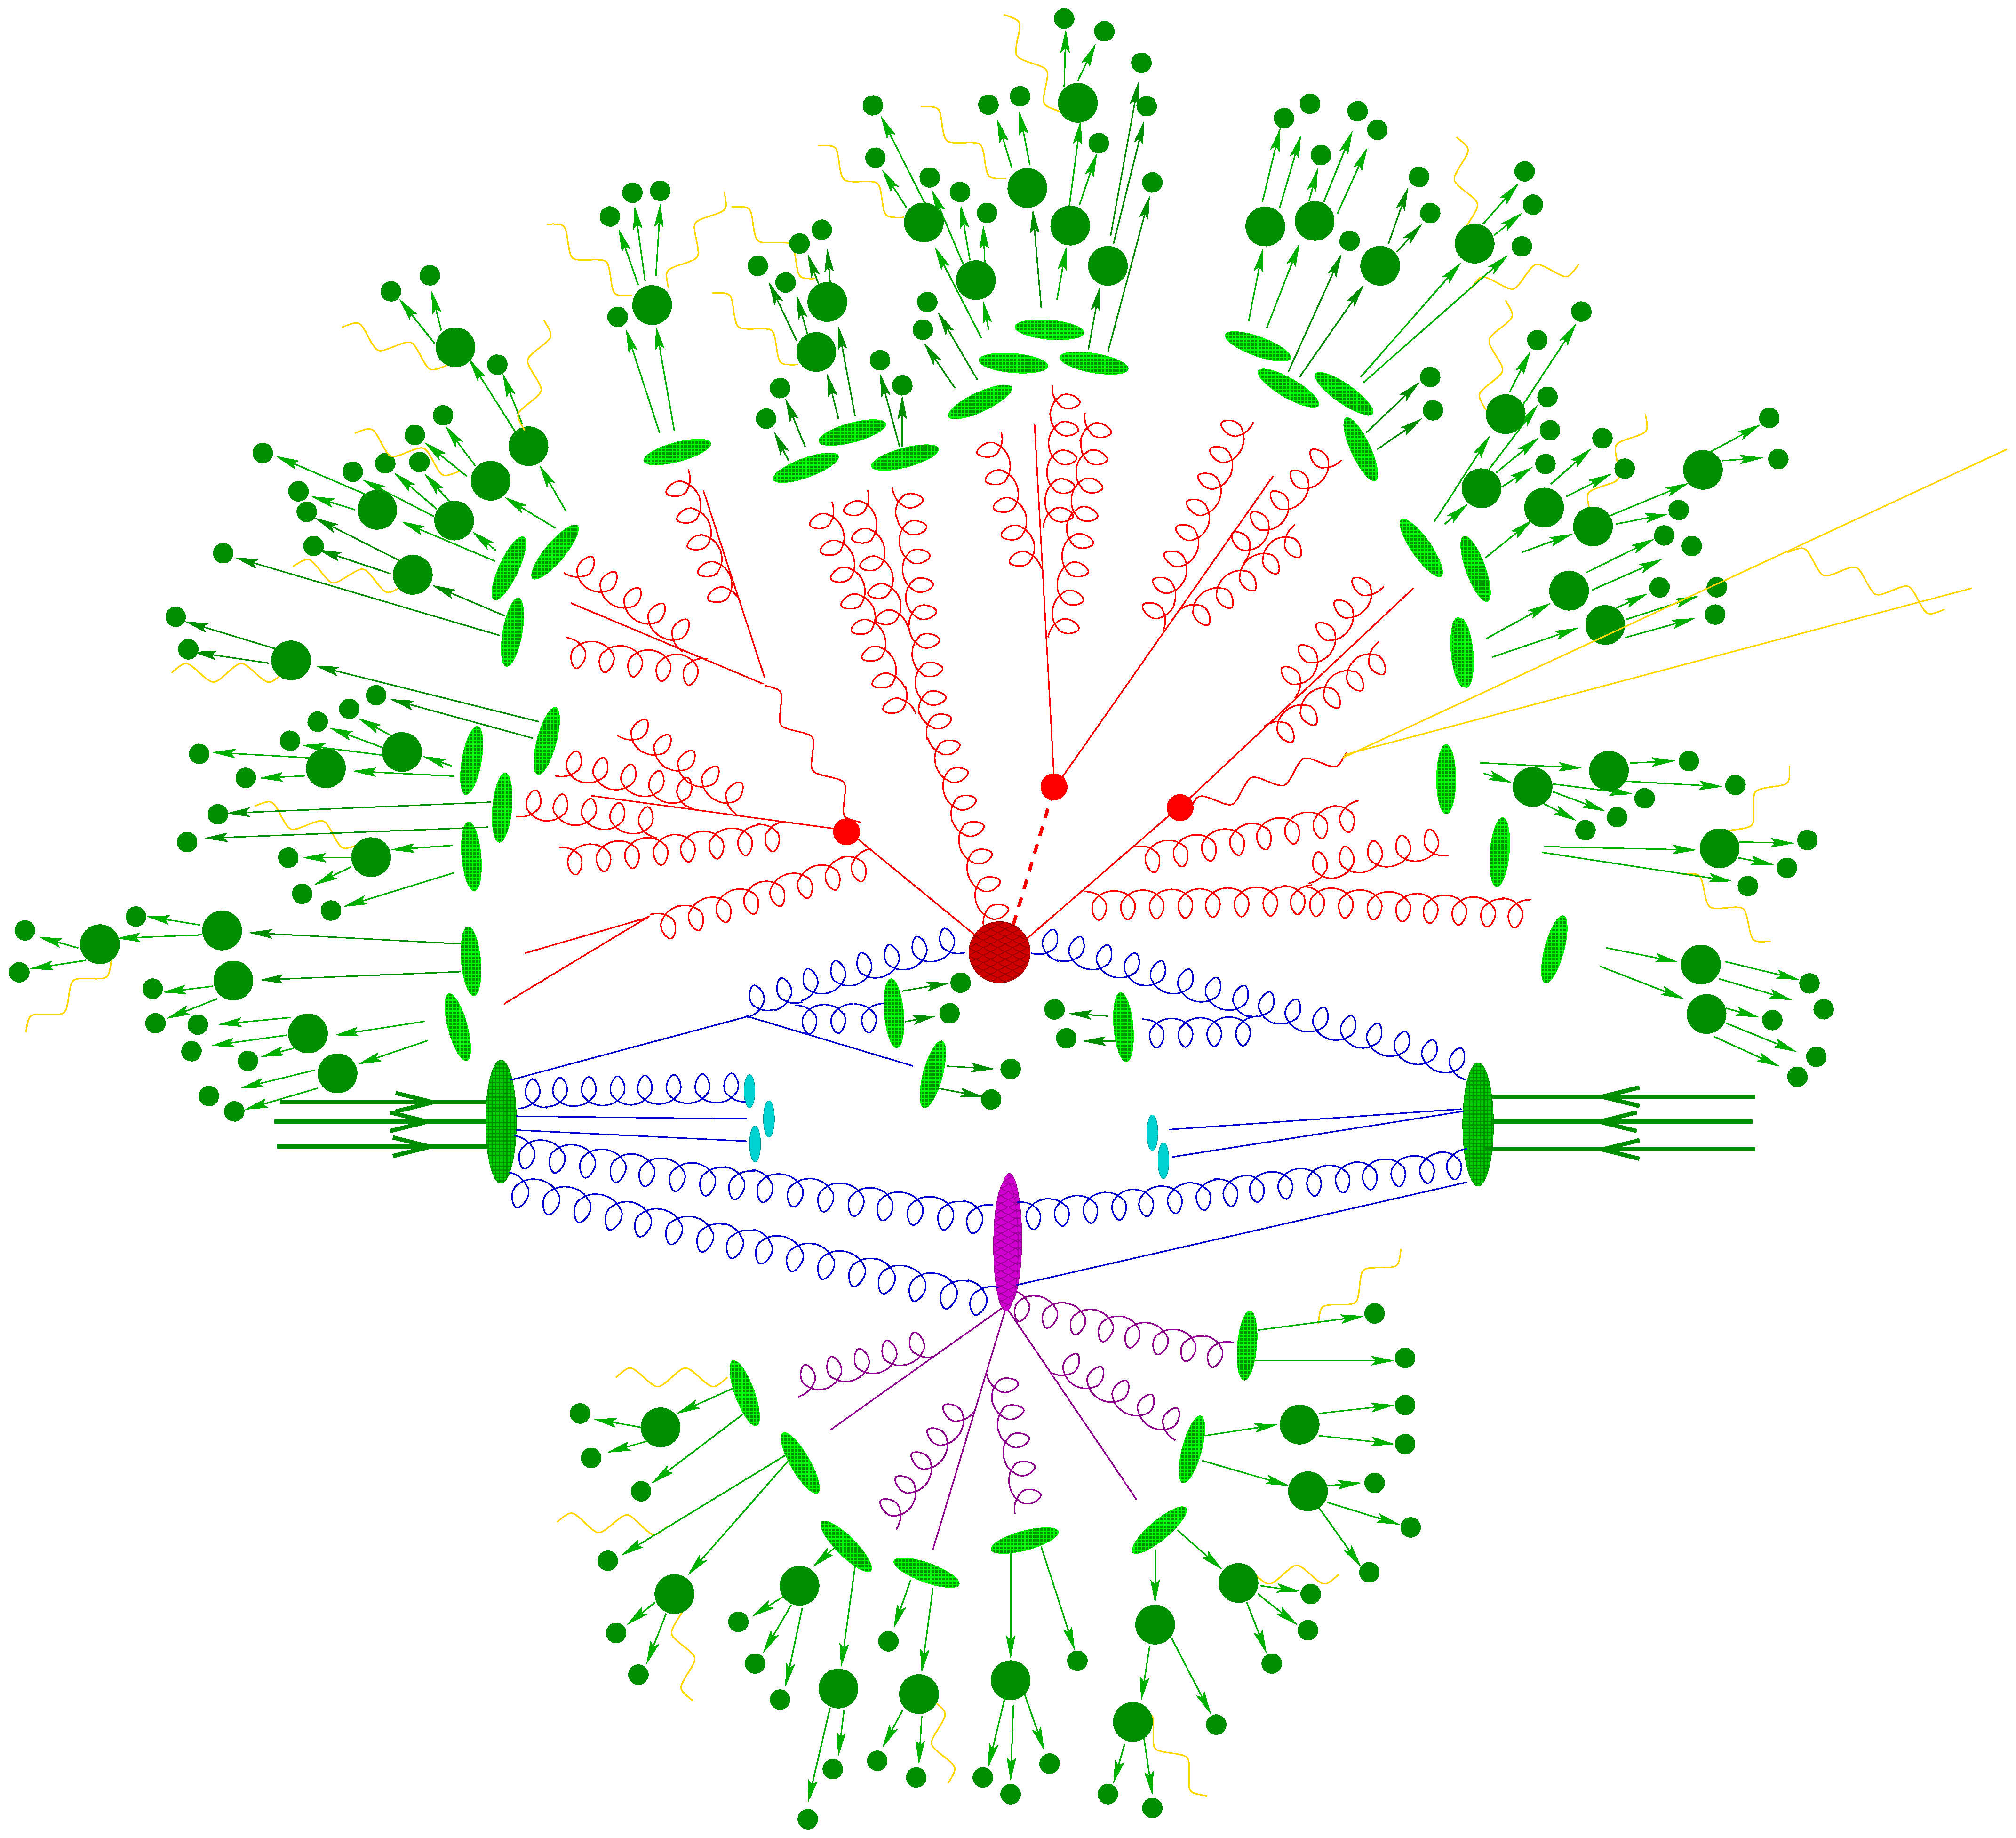
\includegraphics[width=\textwidth]{collision.eps}
\end{figure}
\end{columns}
\end{frame}
